\documentclass[]{article}
\usepackage{lmodern}
\usepackage{amssymb,amsmath}
\usepackage{ifxetex,ifluatex}
\usepackage{lmodern}
\usepackage{amssymb,amsmath}
\usepackage{ifxetex,ifluatex}
\usepackage{tabularx}
\usepackage{supertabular}
\usepackage{lscape}
\usepackage{multirow}
\usepackage{rotating}
\usepackage{adjustbox}
\usepackage{supertabular}
\usepackage{lscape}
\usepackage{multirow}
\usepackage{tabularx}
\usepackage{csquotes}
\usepackage{upgreek}
\usepackage{hyperref}
\usepackage{lineno}
\usepackage{rotating}
\usepackage{adjustbox}
\usepackage{booktabs}
\usepackage{fixltx2e} % provides \textsubscript
\ifnum 0\ifxetex 1\fi\ifluatex 1\fi=0 % if pdftex
  \usepackage[T1]{fontenc}
  \usepackage[utf8]{inputenc}
\else % if luatex or xelatex
  \ifxetex
    \usepackage{mathspec}
  \else
    \usepackage{fontspec}
  \fi
  \defaultfontfeatures{Ligatures=TeX,Scale=MatchLowercase}
\fi
% use upquote if available, for straight quotes in verbatim environments
\IfFileExists{upquote.sty}{\usepackage{upquote}}{}
% use microtype if available
\IfFileExists{microtype.sty}{%
\usepackage{microtype}
\UseMicrotypeSet[protrusion]{basicmath} % disable protrusion for tt fonts
}{}
\usepackage[margin=1in]{geometry}
\usepackage{hyperref}
\hypersetup{unicode=true,
            pdftitle={Study 1C analyses},
            pdfborder={0 0 0},
            breaklinks=true}
\urlstyle{same}  % don't use monospace font for urls
\usepackage{graphicx,grffile}
\makeatletter
\def\maxwidth{\ifdim\Gin@nat@width>\linewidth\linewidth\else\Gin@nat@width\fi}
\def\maxheight{\ifdim\Gin@nat@height>\textheight\textheight\else\Gin@nat@height\fi}
\makeatother
% Scale images if necessary, so that they will not overflow the page
% margins by default, and it is still possible to overwrite the defaults
% using explicit options in \includegraphics[width, height, ...]{}
\setkeys{Gin}{width=\maxwidth,height=\maxheight,keepaspectratio}
\IfFileExists{parskip.sty}{%
\usepackage{parskip}
}{% else
\setlength{\parindent}{0pt}
\setlength{\parskip}{6pt plus 2pt minus 1pt}
}
\setlength{\emergencystretch}{3em}  % prevent overfull lines
\providecommand{\tightlist}{%
  \setlength{\itemsep}{0pt}\setlength{\parskip}{0pt}}
\setcounter{secnumdepth}{0}
% Redefines (sub)paragraphs to behave more like sections
\ifx\paragraph\undefined\else
\let\oldparagraph\paragraph
\renewcommand{\paragraph}[1]{\oldparagraph{#1}\mbox{}}
\fi
\ifx\subparagraph\undefined\else
\let\oldsubparagraph\subparagraph
\renewcommand{\subparagraph}[1]{\oldsubparagraph{#1}\mbox{}}
\fi

%%% Use protect on footnotes to avoid problems with footnotes in titles
\let\rmarkdownfootnote\footnote%
\def\footnote{\protect\rmarkdownfootnote}

%%% Change title format to be more compact
\usepackage{titling}

% Create subtitle command for use in maketitle
\providecommand{\subtitle}[1]{
  \posttitle{
    \begin{center}\large#1\end{center}
    }
}

\setlength{\droptitle}{-2em}

  \title{Study 1C analyses}
    \pretitle{\vspace{\droptitle}\centering\huge}
  \posttitle{\par}
  \subtitle{ED6}
  \author{}
    \preauthor{}\postauthor{}
      \predate{\centering\large\emph}
  \postdate{\par}
    \date{2020-05-01}


\begin{document}
\maketitle

\hypertarget{plot}{%
\subsection{a}\label{plot}}

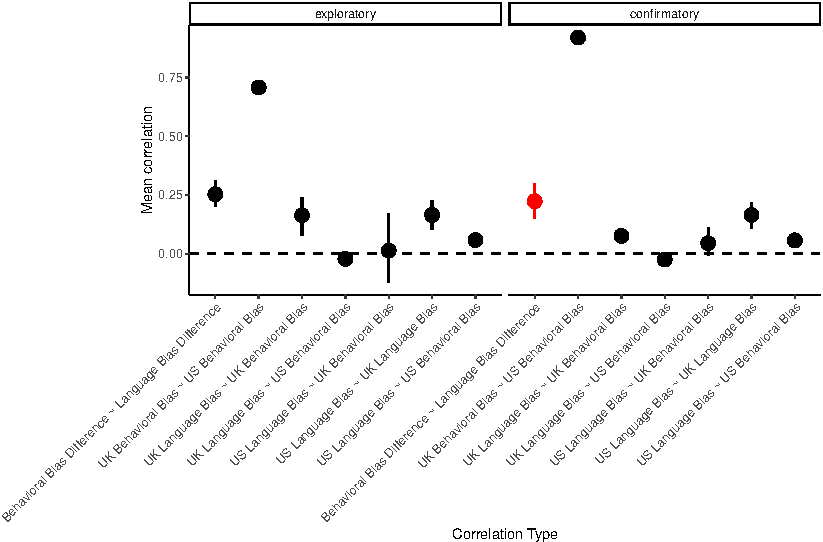
\includegraphics{ED7_files/figure-latex/unnamed-chunk-3-1.pdf}

\hypertarget{mixed-effect-model}{%
\subsection{b}\label{mixed-effect-model}}

\begin{table}[h]
\centering
\begin{tabular}{|l|l|l|l|}
\hline

& \bf{Behavioral Effect Resid} & & \\ \hline
\bf{Predictors} & Estimate & SE & Statistic \\ \hline
(intercept) & -0.00 & 0.05 & -0.09 \\ \hline
country (uk) & 0.02 & 0.01 & 1.74 \\ \hline
language bias difference (uk - us) & -0.03 & 0.07 & -0.42 \\ \hline
country:language bias difference & 0.05 & 0.02 & 2.88 \\ \hline
\bf{Random Effects} \\ \hline
s2 & 0.20  & & \\ \hline
T00 user id & 0.01  & & \\ \hline
T00 domain & 0.07 & &  \\ \hline
N user id & 22059  & & \\ \hline
N domain & 31  & & \\ \hline
\specialrule{.1em}{.05em}{.05em} 
Observations & 27045  & & \\ \hline

\end{tabular}
\end{table}

\hypertarget{title-and-legend}{%
\subsection{Title and Legend}\label{title-and-legend}}

Study 1c models

a, The exact pre-registered analysis (\url{https://osf.io/3f9ed/}) of Study 1c is presented. Pairwise correlations between all variables
(language bias, behavioral bias, and UK-US difference measures) are shown, averaging across estimates of language bias from the 5 model runs. Error bars are 95\% CIs. As stated in the pre-registration, the key test of our hypothesis is that the correlation between the UK - US linguistic difference (``Language Bias Difference'') and the UK - US behavioral difference (``Behavioral Bias Difference'') is greater than 0 (shown in red). That data are consistent with this prediction. The confirmatory dataset is shown on the right, along with the smaller exploratory dataset on the left for reference. b,The full results to the mixed-effect model described in the paper are presented.


\end{document}
